\documentclass[14pt]{extarticle}

\let\Overrightarrow\overrightarrow
\let\vecarrow\overrightarrow


%other%
\usepackage{graphicx}
\usepackage{float}
\usepackage[margin=0.7in]{geometry}
\usepackage{caption}
\usepackage{csquotes}
\usepackage[export]{adjustbox}
\usepackage{wrapfig}
\usepackage{setspace}
\usepackage{anyfontsize}
\usepackage{titlesec}
\titleformat{\section}{
	\normalfont\fontsize{20}{20}\bfseries}{\thesection}{1em}{}
\titleformat{\subsection}{
	\normalfont\fontsize{17}{20}\bfseries}{\thesubsection}{0.1em}{}
\usepackage{relsize}
%other%



%%\newcommand{\F}{\Oldmathbfcal{F}}
%math%
\usepackage{amsthm}
\usepackage{amssymb}
\usepackage{amsmath}
\usepackage{mathtools}
%%\usepackage[cal = pxtx, scr = dutchcal]{mathalfa}



%\usepackage{unicode-math}
%\newtheorem*{}{\textup{Лемма}}
\newtheorem*{theorem}{\textup{Теорема}}
\newtheorem*{remark}{\textup{Комментарий}}
%\renewcommand\qedsymbol{$\blacksquare$}
%\usepackage{parskip}

\usepackage{pgfplots}
\usepgfplotslibrary{polar}
\usepgflibrary{shapes.geometric}
\usetikzlibrary{calc}


\renewenvironment{proof}
    {\noindent \textit{Доказательство.}\\
	\indent $\square$}
	{ $\blacksquare$\\ }

\newenvironment{solution}
	{\vspace{-4.3mm} \noindent\textbf{Решение.}}


\renewenvironment{remark}
    {\noindent\textbf{Коментарий}}

\usepackage{tikz}
   \usetikzlibrary{calc}

\newcommand{\arc}[0]{
   \tikz [baseline = (N.base), every node/.style={}] {
	  \node [inner sep = 0pt] (N){}; %{$#0$};
      \draw [line width = 0.8pt] plot [smooth, tension=1.3] coordinates {
         ($(N.north west) + (-1.5ex,0.6ex+0.4ex)$)
         ($(N.north)      + (-0.75ex,0+0.4ex)$)
         ($(N.north east) + (0ex,0.6ex+0.4ex)$)
      };
   }
}

\renewenvironment{rcases}
  {\left.\begin{aligned}}
  {\end{aligned}\right\rbrace}

\DeclarePairedDelimiter\abs{\lvert}{\rvert}
\DeclarePairedDelimiter\norm{\lVert}{\rVert}

%\newcounter{example}[section]
\newenvironment{example}[1]{\noindent \textbf{Пример #1.}}

\let\mathb\mathbb


\newcommand{\N}{\mathb{N}}
\newcommand{\Z}{\mathb{Z}}
\newcommand{\R}{\mathb{R}}
\newcommand{\F}{\mathbfcal{F}}
\renewcommand{\P}{\mathbfcal{P}}
%\newcommand*{\Z}{\mathbb{Z}}
%math%

%fonts%
\usepackage[russian]{babel}
\usepackage{polyglossia}
\setdefaultlanguage[spelling=modern]{russian}
%\setotherlanguage{english}
\setmainfont{CMU Serif}
\setsansfont{CMU Sans Serif}
\setmonofont{CMU Typewriter Text}  
%\setmathfont{Latin Modern Math}
\usepackage{mathrsfs}
%\DeclareMathAlphabet{\mathcal}{T1}{TX}{m}{n}

\usepackage{unicode-math}


%\let\Oldmathbfcal=\mathbfcal
%\renewcommand{\mathbfcal}{\mumble\Oldmathbfcal}

%%\newcommand{\F}{\Oldmathbfcal{F}}
%%\newcommand{\F}{𝓕}

%\usepackage{fontspec}
\setmathfont{Latin Modern Math}

\DeclareSymbolFont{symbols}{OMS}{cmsy}{m}{n}
\DeclareSymbolFont{bsymbols}{OMS}{cmsy}{b}{n}
\DeclareSymbolFontAlphabet{\mathcal}{symbols}
\DeclareSymbolFontAlphabet{\mathbfcal}{bsymbols}

%\setmathfont[range = {2131}]{AMS}
%\usepackage{amsfonts}
%\usepackage{dsfont}
%fonts%


\begin{document}

\textbf{\textit{Условие.}} Точки \(A_1\), \(B_1\), \(C_1\) --- середины сторон соответственно \(BC\), \(AC\), \(AB\) 
треугольника \(ABC\), а \(BH\) -- его высота. 
Докажите, что если описанные окружности 
треугольников \(AHC_1\) и \(CHA_1\) проходят через 
точку \(M\), то \(\angle ABM = \angle CBB_1\).

\begin{figure}[H]
    \centering
    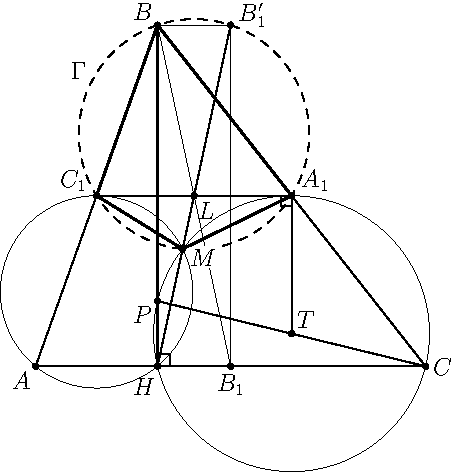
\includegraphics[height=12cm]{fig.pdf}
\end{figure}

\textbf{\textit{Решение.}} Ясно, что изначальное условие равносильно тому, что
точка \(M\) находится на симедиане треугольника 
\(ABC\) -- это и будем доказывать.
Сперва покажем, что обе окружности \((AHC_1)\) и \((CHA_1)\) 
касаются прямой \(A_1C_1\). Действительно, для окружности \((CHA_1)\) 
имеем: \(P = BH \cap (CHA_1) \), \(T\) -- середина
\(PC\); тогда \(T\) -- центр нашей окружности, 
кроме того \(TA_1\) -- средняя линия треугольника 
\(CPB\), а следовательно прямая \(TA_1\) 
перпендикулярна \(C_1A_1\), что и означает касание. Аналогично доказывается и для \((AHC_1)\). Далее, пусть \(L\) -- середина отрезка \(A_1C_1\), 
тогда, так как окружности касаются его в точках 
\(A_1\) и \(C_1\), то \(MH\) проходит через \(L\).
Пусть \(\Gamma = (A_1C_1B)\), тогда \(M \in \Gamma\). Так как треугольник 
\(BA_1C_1\) гомотетичен \(BCA\) с центром гомотетии в вершине \(B\), то 
прямые \(BM\) и \(BL\) для треугольника \(BA_1C_1\) 
--- симедиана и медиана 
соответственно. А значит осталось доказать, что четырёхугольник \(A_1BC_1M\) -- гармонический. 

Теперь заметим, что \(\Gamma\) симметрична окружности Эйлера треугольника \(ABC\) относительно прямой \(A_1C_1\). 
А значит, отразив \(B_1\) относительно \(A_1C_1\), мы 
получим точку \(B_1' \in \Gamma\). Так как 
\(HBB_1'B_1\) -- прямоугольник, то это означает, 
что \(B_1'\) симметрична \(B\) относительно серединного 
перпендикуляра к \(A_1C_1\). Просуммируем вышесказанное в лемму. \\


%\pagebreak

\textbf{\textit{Лемма.}} Пусть дан треугольник \(ABC\), 
\(M\) -- середина его стороны \(AC\), \(B'\) симметрична \(B\) относительно серединного перпендикуляра \(\ell\) к отрезку \(AC\) 
(очевидно лежит на \((ABC)\)), \(D\) -- вторая точка 
пересечения прямой  \(B'M\) с окружностью \((ABC)\). Тогда четырёхугольник \(ABCD\) -- гармонический.\\

\textbf{\textit{Доказательство.}}\\
\textbf{\textit{Первый способ.}} 
Пусть \(W\) -- середина дуги \(ABC\). Тогда 
\(\arc WB = \arc WB'\), ведь \(B\) и \(B'\) 
симметричны относительно \(\ell\) .
%\(\arc WB = \arc ABC/2 - \arc BA = \arc ABC/2 - 
%\arc B'C =\arc WB'\), 
Отсюда следует, что \(DB\) -- симедиана треугольника 
\(DAC\), а это равносильно тому, что \(ABCD\) -- гармонический.

\begin{figure}[H]
    \centering
    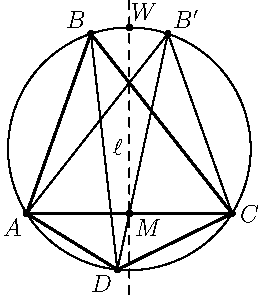
\includegraphics[height=8cm]{fig2.pdf}
\end{figure}




\textbf{\textit{Второй способ.}} 

\indent Условие задачи 
равносильно тому, что \(AB \cdot DC = AD \cdot BC\).

Из подобия треугольников \(ADM\) и \(B'MC\) 
получаем, что \(\dfrac{AD}{B'C} = \dfrac{AM}{MB'}\), 
а из подобия реугольников \(DMC\) и \(AMB'\):
\(\dfrac{CD}{AB'} = \dfrac{CM}{MB'}\). Откуда 
\(\dfrac{AD}{B'C} = \dfrac{CD}{AB'}\). Так как 
из симметрии \(CB = AB'\) и \(B'C = AB\), то это 
равносильно следующему 
\(\dfrac{AD}{AB} = \dfrac{CD}{BC}\), что и 
требовалось.




\end{document}
